\iffalse
    \author{EE24BTECH11061}
    \section{ae}
    \chapter{2016}
 \fi
%\begin{enumerate}
\item The chairman requested the aggrieved shareholders to \rule{1cm}{0.15mm} him.
\begin{multicols}{2}
    \begin{enumerate}
        \item bare with
        \item bore with
        \item bear with
        \item bare
    \end{enumerate}
\end{multicols}

\item Identify the correct spelling out of the given options:
\begin{multicols}{1}
    \begin{enumerate}
        \item Managable
        \item Manageable
        \item Mangaeble
        \item Managible
    \end{enumerate}
\end{multicols}

\item Pick the odd one out in the following:\\
13, 23, 33, 43, 53
\begin{multicols}{1}
    \begin{enumerate}
        \item 23
        \item 33
        \item 43
        \item 53
    \end{enumerate}
\end{multicols}

\item R2D2 is a robot. R2D2 can repair aeroplanes , No other robot can repair aeroplanes.\\
Which of the following can be logically inferred from the above statements?
\begin{multicols}{2}
    \begin{enumerate}
        \item R2D2 is a robot which can only repair aeroplanes.
        \item R2D2 is the only robot which can repair aeroplanes.
        \item R2D2 is a robot which can repaie only aeroplanes.
        \item Only R2D2 is a robot.
    \end{enumerate}
\end{multicols}

\item If $\abs{9y - 6} = 3$, then $y^2 - 4y/3$ is \rule{1cm}{0.15mm}
\begin{multicols}{2}
    \begin{enumerate}
        \item 0
        \item +1/3
        \item -1/3
        \item undefined
    \end{enumerate}
\end{multicols}

\item The following graph represents the installed capacity for cement production (in tonnes) and the
actual production (in tonnes) of nine cement plants of a cement company. Capacity utilization of a
plant is defined as ratio of actual production of cement to installed capacity. A plant with installed
capacity of at least 200 tonnes is called a large plant and a plant with lesser capacity is called a
small plant. The difference between total production of large plants and small plants, in tonnes is \rule{1cm}{0.15mm}.
\begin{figure}
    \centering
    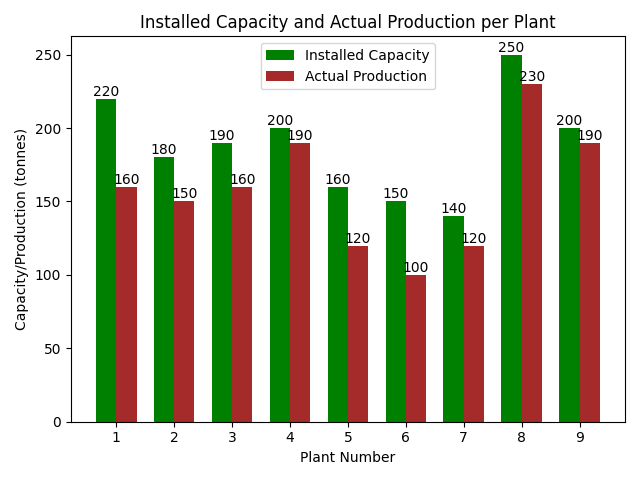
\includegraphics[width=0.5\linewidth]{GATE-yearwise/2016/S1/figs/figure.png}
    \label{fig:enter-label}
\end{figure}

\item A poll of students appearing for masters in engineering indicated that 60\% of the students believed that mechanical engineering is a profession unsuitable for women. A research study on women with
masters or higher degrees in mechanical engineering found that 99\% of such women were successful in their professions.\\
Which of the following can be logically inferred from the above paragraph?
\begin{enumerate}
    \item Many students have misconceptions regarding various engineering disciplines.
    \item Men with advanced degrees in mechanical engineering believe women are well suited to be mechanical engineers.
    \item Mechanical engineering is a profession well suited for women with masters or higher degrees in mechanical engineering.
    \item The number of women pursuing higher degrees in mechanical engineering is small.
\end{enumerate}

\item Sourya committee had proposed the establishment of Sourya Institutes of Technology (SITs) in line with Indian Institutes of Technology (IITs) to cater to the technological and industrial needs of a developing country. \\
Which of the following can be logically inferred from the above sentence?\\
Based on the proposal,
\begin{enumerate}[label = (\roman*)]
    \item In the initial years, SIT students will get degrees from IIT.
    \item SITs will have a distinct national objective.
    \item SIT like institutions can only be established in consultation with IIT.
    \item SITs will serve technological needs of a developing country.
\end{enumerate}
\begin{multicols}{2}
    \begin{enumerate}
        \item (iii) and (iv) only.
        \item (i) and (iv) only. 
        \item (ii) and (iv) only. 
        \item (ii) and (iii) only. 
    \end{enumerate}
\end{multicols}

\item Shaquille O' Neal is a 60\% career free throw shooter, meaning that he successfully makes 60 free throws out of 100 attempts on average. What is the probability that he will successfully make \underline{exactly} 6 free throws in 10 attempts? 
\begin{multicols}{2}
    \begin{enumerate}
        \item 0.2508
        \item 0.2816
        \item 0.2934
        \item 0.6000
    \end{enumerate}
\end{multicols}

\item The numerical in the units position of $211^{870} + 146^{127} \times 3^{424}$ is \rule{1cm}{0.15mm} .
%\end{enumerate}